\documentclass[12pt,oneside]{scrartcl}
\usepackage[a4paper, left=2.5cm, right=2cm, top=5.5cm, bottom=2.5cm]{geometry}
\usepackage[ngerman]{babel}
\usepackage{color}
\usepackage[utf8]{inputenc}
\usepackage{amsmath}
\usepackage{amsfonts}
\usepackage{amssymb}
\usepackage{siunitx}
\usepackage{graphicx}
\usepackage{pgfplots}
\usepackage{hyperref}
\sisetup{locale = DE}
\newcommand{\phyphox}{\textit{phyphox} }
\usepackage{biblatex}
\usepackage{xltabular}
\addbibresource{Schallgeschwindigkeit.bib}
\usepackage{scrlayer-scrpage}
\newcolumntype{C}[1]{>{\centering\arraybackslash}p{#1}}
\DeclareNewLayer[%
  background,% Hintergrundebene
  width=\textwidth,% Größe und Position des Textbereichs
  hoffset=2.5cm,
  voffset=2.5cm,
  align=tl,
  contents={%
  \sffamily
    \setlength{\fboxsep}{2mm}% Abstand Box Text
    \setlength{\fboxrule}{.5mm}% Dicke Linie
    % vertikale Position korrigieren    
    \vskip-\fboxsep\vskip-\fboxrule\vskip-\baselineskip
    % horizontale Position korrigieren
    \hspace{-\fboxsep}\hspace{-\fboxrule}%
        
    \begin{tabularx}{\textwidth}{|>{\bfseries\Large}C{7cm}|X|X|}                                                       
\hline
\vspace{0em}
\includegraphics[scale=0.3]{logo2.png} & Name: & Datum: \\
\hline

\end{tabularx}
    %\makebox[\layerwidth][l]{%
    %  \fbox{\rule{0pt}{\layerheight}\rule{\layerwidth}{0pt}}% Rahmen
    %}%
  }
]{frame}
\AddLayersToPageStyle{@everystyle@}{frame}

\begin{document}
\sffamily

\title{Mechanische Wellen}
\subtitle{Experiment Bestimmung der Schallgeschwindigkeit}
\date{}
\maketitle
\section*{Versuchsbeschreibung}
Mit zwei Smartphones kann zusammen mit einer zweiten Person im Unterricht oder zu Hause die Schallgeschwindigkeit bestimmt werden. Die App \phyphox\footnote{Die App \phyphox wird von der RWTH Aachen entwickelt und steht allen Interessierten \textbf{kostenlos} zur Verfügung. \phyphox ermöglicht es dir, mit den Sensoren deines Smartphones zu experimentieren, Messwerte aufzunehmen und auszuwerten.}  auf den beiden Smartphones bestimmt dabei die Zeitspanne, die der Schall benötigt, um eine vorgegebene Strecke zu durchlaufen.
\section*{Material}
Außer zwei Smartphones, auf dem die App \phyphox installiert ist, wird noch ein Maßband benötigt.
\section*{Versuchsaufbau}
Beide Experimentatoren platzieren Ihre Smartphones in einem gemessenen Abstand $s$ von mindestens \SI{5}{\meter} voneinander entfernt und stellen sich jeweils hinter ein Smartphone, so dass die Smartphones zwischen beiden Personen liegen (siehe \autoref{fig1}).
\begin{figure}[ht]
	\centering
  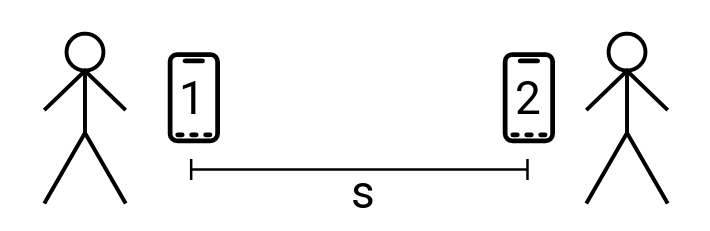
\includegraphics[width=0.66\textwidth]{Messung.png}
	\caption{{\small Versuchsanordnung zur Messung der Schallgeschwindigkeit mit zwei Personen und zwei Smartphones \texttt{akustische Stoppuhr}.}}
	\label{fig1}
\end{figure}
\section*{Versuchsdurchführung}
\begin{enumerate}
\item Bestimmen Sie den Abstand der beiden Smartphones
\item Starten Sie auf beiden Smartphones die App \phyphox und wählen Sie die Messung \texttt{akustische Stoppuhr}
\item Stellen Sie unter der Kategorie \texttt{Einfach} die Schwelle so ein, dass die Stoppuhr nicht von selbst auslöst.
\item Nun klatscht erst einer in die Hände, so dass das Geräusch beide Stoppuhren startet.
\item Anschließend klatscht die andere Person in die Hände, um beide Uhren wieder zu stoppen.
\end{enumerate}
\subsection*{Hinweise zur Durchführung}
\begin{itemize}
\item \textbf{Wichtig ist hierbei, dass das Geräusch möglichst auf der Höhe des Smartphones erzeugt wird, damit die Schallwelle von der Quelle auf einer möglichst geraden Linien über beide Smartphones hinweg läuft.}
\item \textbf{Die Messung wird um so genauer, je größer die Strecke ist, die der Schall durchlaufen muss.}
\item \textbf{Damit das Klatschen über eine große Entfernung die Stoppuhr des zweiten Smartphones exakt starten und stoppen kann, muss es also möglichst ruhig sein.}
\end{itemize}
\section*{Aufgaben}
\begin{enumerate}
\item Wiederholen Sie die Messung 5 mal und tragen Sie ihre Messwerte in die folgende Tabelle ein\\\\
\vspace{0,5cm}
\begin{large}
\begin{tabular}{|c|c|c|c|}
\hline
Messung Nr. & Zeitspanne A  & Zeitspanne B & Schallgeschwindigkeit \\
 & $\Delta t_{A}$ in s &  $\Delta t_{B}$ in s & $v$ in $\si{\meter\per\second}$ \\ 
\hline 
1 &  &  & \\ 
\hline 
2 &  &  & \\ 
\hline 
3 &  &  & \\ 
\hline 
4 &  &  & \\ 
\hline 
5 &  &  & \\ 
\hline 
\hline
\multicolumn{3}{|c|}{Abstand $s$ in $\si{\meter}$} &  \\
\hline
\multicolumn{3}{|c|}{mittlere Schallgeschwindigkeit $\overline{v}$ in \si{\meter\per\second}} & \\
\hline
\end{tabular}\label{tab}\end{large} \\
\item Berechnen Sie die Schallgeschwindigkeit mit den gemessenen Werten.
\end{enumerate}

\section*{Bestimmung der Schallgeschwindigkeit}
\begin{enumerate}
\item Darstellung der Messgrößen im $t-x$-Diagramm.\\
  \begin{tikzpicture}
  \begin{scope}[scale=0.013]
    \draw [->, >=latex, thick] (0,0) -- (0,400) node [left] {$x$};
    \draw [->, >=latex, thick] (0,0) -- (550,0) node [below] {$t$};
    \draw [red, thick](50,0) node [below, green] {$t_{A,Start}$} -- (150,350);
    \draw [red, thick](350,350) -- (450,0) node [below, green] {$t_{A,Stop}$};
    \draw [very thin, black!60] (150,-5) -- (150,350);
    \draw [very thin, black!60] (350,-5) -- (350,350);
    \node [cyan] at (150,-30) {$t_{B,Start}$};
    \node [cyan] at (350,-30) {$t_{B,Stop}$};
    \draw [<->, >=latex, thick, red] (-60,0) -- node [midway, left] {$s$} (-60,350);
    \node [green] at (-20,0) {$x_{A}$};
    \node [cyan] at (-20,350) {$x_{B}$};
    \draw [<->, >=latex, thick, green] (50,-75) -- node [midway, above] {$\Delta t_A$} (450,-75);
    \draw [<->, >=latex, thick, red] (50,-130) -- node [midway, above] {$\Delta t$} (150,-130);
    \draw [<->, >=latex, thick, red] (350,-130) -- node [midway, above] {$\Delta t$} (450,-130);
    \draw [<->, >=latex, thick, cyan] (150,-130) -- node [midway, above] {$\Delta t_B$} (350,-130);
  \end{scope}
  \end{tikzpicture}
  \begin{description}
  \item[$x_A$:\quad] Ort von Smartphone A
  \item[$x_B$:\quad] Ort von Smartphone B
  \item[$s$:\quad] Abstand der beiden Smartphones
  \item[$t_{A,Start}$:\quad] Zeitpunkt des Starts von Smartphone A
  \item[$t_{A,Stop}$:\quad] Zeitpunkt des Stopps von Smartphone A
  \item[$\Delta t_A$:\quad] Zeitspanne, die Smartphone A misst
  \item[$t_{B,Start}$:\quad] Zeitpunkt des Starts von Smartphone B
  \item[$t_{B,Stop}$:\quad] Zeitpunkt des Stopps von Smartphone B
  \item[$\Delta t_B$:\quad] Zeitspanne, die Smartphone B misst
  \item[$\Delta t$:\quad] Zeitspanne, die der Schall benötigt, um von Smartphone A zu Smartphone B zu gelangen
  \end{description}

\item Bezeichnen wir mit $x_A$ den Ort von Smartphone A und mit $x_B$ den Ort von Smartphone B, dann ist $s = x_B - x_a$ der Abstand der beiden Smartphones.\\\\
Bezeichnen wir weiter mit $t_{A,Start}$ den Zeitpunkt des Starts von Smartphone A, $t_{B,Start}$ den Zeitpunkt des Starts von Smartphone B, $t_{A,Stop}$ den Zeitpunkt des Stopps von Smartphone A und $t_{B,Stop}$ den Zeitpunkt des Stopps von Smartphone B, dann ist $\Delta t_A = t_{A,Stop} - t_{A,Start}$ die Zeitspanne, die Smartphone A misst und $\Delta t_B = t_{B,Stop} - t_{B,Start}$ die Zeitspanne, die Smartphone B misst.
Bezeichnen wir schließlich mit $\Delta t$ die Zeitspanne, die der Schall benötigt, um von Smartphone A zu Smartphone B (und umgekehrt) zu gelangen, so entnimmt man aus dem $t-x$-Diagramm
\begin{align*}
\Delta t_A&=\Delta t+\Delta t_B +\Delta t\\
\Leftrightarrow \Delta t_A&=\Delta t_B + 2\cdot\Delta t\\
\Leftrightarrow \Delta t_A-\Delta t_B&=2\cdot\Delta t\\
\Leftrightarrow \dfrac{\Delta t_A-\Delta t_B}{2}&=\Delta t
\end{align*}
Damit ergibt sich für die Schallgeschwindigkeit $v$
\begin{align*}
v=\dfrac{s}{\Delta t}=\dfrac{s}{\frac{\Delta t_A-\Delta t_B}{2}}=\dfrac{2\cdot s}{\Delta t_A-\Delta t_B}\\
\\
\boxed{v=\dfrac{2\cdot s}{\Delta t_A-\Delta t_B}}
\end{align*}
\end{enumerate}
\end{document}